% =============================================================================
% Outer cover template — KDP 6" x 9" paperback (standalone, do not \input)
% Replicates dimensions of PAPERBACK_6.000x9.000_110_BW_WHITE_en_US template.
% Compile with XeLaTeX. Works from template dir or project root:
%   From template dir:  xelatex outer-cover-template.tex
%   From project root:  xelatex -output-directory="cover-template 6x9 in/out" "cover-template 6x9 in/outer-cover-template.tex"
% =============================================================================

\documentclass[11pt]{article}

% KDP template: "12.498" x 9.250" Overall Dimensions" (317.44mm x 234.95mm)
\usepackage[
  paperwidth=12.498in,
  paperheight=9.25in,
  margin=0in,
  headheight=0pt,
  headsep=0pt,
  footskip=0pt,
]{geometry}

% Cover-only preamble: fonts, \jcz, \ruby — no document class, no book-only stuff
\usepackage{import}
\subimport{}{cover-preamble.tex}

\usepackage{tikz}

% -----------------------------------------------------------------------------
% Dimensions (inches) — from KDP PAPERBACK_6.000x9.000_110_BW_WHITE_en_US.pdf
% -----------------------------------------------------------------------------
\newlength{\bleed}
\setlength{\bleed}{0.125in}       % KDP bleed on all sides (red area = bleed)

\newlength{\trimwidth}
\setlength{\trimwidth}{6in}       % trim size width per panel (152.40mm)

\newlength{\trimheight}
\setlength{\trimheight}{9in}      % trim size height (228.60mm)

\newlength{\spinewidth}
\setlength{\spinewidth}{0.248in}  % KDP: "0.248" Spine Width" for 110 pp white (6.29mm)

\newlength{\safemargin}
\setlength{\safemargin}{0.125in} % inner margin inside trim: keep text/logos inside live area (inner pink band)

% Derived: total width = left bleed + back + spine + front + right bleed
%          = 0.125 + 6 + 0.248 + 6 + 0.125 = 12.498 in
% Total height = 9 + 0.125 + 0.125 = 9.25 in
% Spine fold: blue dashed in KDP; front trim starts at 6.125 + 0.248 = 6.373 in

\pagestyle{empty}
\setlength{\parindent}{0pt}

\begin{document}
\jcz{}
\thispagestyle{empty}


% Full-page cover: 12.498in x 9.25in (KDP overall dimensions)
\begin{tikzpicture}[
  x=1in,
  y=1in,
  every node/.style={inner sep=0pt, outer sep=0pt},
]
  \useasboundingbox (0,0) rectangle (12.498,9.25);

  % % --- Panels (left to right: back cover | spine | front cover) ---
  % % X: [0, 0.125) bleed | [0.125, 6.125) back trim | [6.125, 6.373) spine | [6.373, 12.373) front trim | [12.373, 12.498) bleed
  % % Y: [0, 0.125) bleed | [0.125, 9.125) trim | [9.125, 9.25) bleed

  % % 1) Red area = Out of Live/Bleed (full page)
  % \fill[color=magenta!30] (0,0) rectangle (12.498,9.25);

  % % 2) Inside trim: inner pink band (safe margin); then white = Live Area
  % \fill[magenta!12] (0.125,0.125) rectangle (6.125,9.125);
  % \fill[white] (0.25,0.25) rectangle (6,9);
  % \fill[magenta!12] (6.125,0.125) rectangle (6.373,9.125);
  % \fill[magenta!12] (6.373,0.125) rectangle (12.373,9.125);
  % \fill[white] (6.498,0.25) rectangle (12.248,9);

  % % 3) Outer edge of bleed
  % \draw[line width=2pt, black] (0,0) rectangle (12.498,9.25);

  % % 4) Trim lines
  % \draw[line width=1.2pt, black] (0.125,0.125) rectangle (6.125,9.125);
  % \draw[line width=1.2pt, black] (6.125,0.125) rectangle (6.373,9.125);
  % \draw[line width=1.2pt, black] (6.373,0.125) rectangle (12.373,9.125);

  % % 5) Spine fold lines
  % \draw[line width=1.5pt, black] (6.125,0) -- (6.125,9.25);
  % \draw[line width=1.5pt, black] (6.373,0) -- (6.373,9.25);

  % 6) Back: Kowloon Publishing logo and name; sample Jyutcitzi (ruby).
  \node[anchor=center, inner sep=0] at (3.125,6.5) {\includegraphics[width=1.25in]{../pics/kowloon-publishing-logo.jpg}};
  \node[anchor=center, align=center, font=\Large\bfseries] at (3.125,5.5) {Kowloon Publishing};
  \node[anchor=center, align=center, font=\Large\bfseries] at (3.125,5.3) {九龍印書館};
  
  

  % \node[anchor=center, align=center, font=\Large\bfseries] at (9.373,6.5) {English: God of Cookery};
  % \node[anchor=center, align=center, font=\Large\bfseries] at (9.373,5.2) {Chinese: 食神};
  % \node[anchor=center, align=center, font=\Large\bfseries] at (9.373,4.2) {: };
  % \node[anchor=center, align=center, font=\Large] at (9.373,3.8) {\ruby{咩}{󰗞}\ruby{話}{󲅕}？\ruby{啊}{󰀒}？\ruby{好}{󱭱}\ruby{野}{󱖜}！};

  % 7) Spine: title vertically stacked at top (y descends)
  \node[anchor=center, font=\scriptsize\sffamily, black, align=center] at (6.249,8.75) {食};
  \node[anchor=center, font=\scriptsize\sffamily, black, align=center] at (6.249,8.5) {神};
  \node[anchor=center, font=\scriptsize\sffamily, black, align=center] at (6.249,8.25) {劇};
  \node[anchor=center, font=\scriptsize\sffamily, black, align=center] at (6.249,8.0) {本};
  \node[anchor=center, font=\scriptsize\sffamily, black, align=center] at (6.249,7.75) {全};
  \node[anchor=center, font=\scriptsize\sffamily, black, align=center] at (6.249,7.5) {文};
  \node[anchor=center, font=\scriptsize\sffamily, black, align=center] at (6.249,7.25) {\jcz{}};
  \node[anchor=center, font=\scriptsize\sffamily, black, align=center] at (6.249,7.0) {\jcz{}};
  \node[anchor=center, font=\scriptsize\sffamily, black, align=center] at (6.249,6.75) {\jcz{}};
  \node[anchor=center, font=\scriptsize\sffamily, black, align=center] at (6.249,6.5) {註};
  \node[anchor=center, font=\scriptsize\sffamily, black, align=center] at (6.249,6.25) {音};


    % Spine: 九龍印書館 at bottom (館 at bottom, stacked up)
  \node[anchor=center, font=\scriptsize\sffamily, black, align=center] at (6.249,1.5) {九};
  \node[anchor=center, font=\scriptsize\sffamily, black, align=center] at (6.249,1.25) {龍};
  \node[anchor=center, font=\scriptsize\sffamily, black, align=center] at (6.249,1.0) {印};
  \node[anchor=center, font=\scriptsize\sffamily, black, align=center] at (6.249,0.75) {書};
  \node[anchor=center, font=\scriptsize\sffamily, black, align=center] at (6.249,0.5) {館};
  


  % Cover art: centered on front panel
  \node[anchor=center, inner sep=0] at (9.373,5) {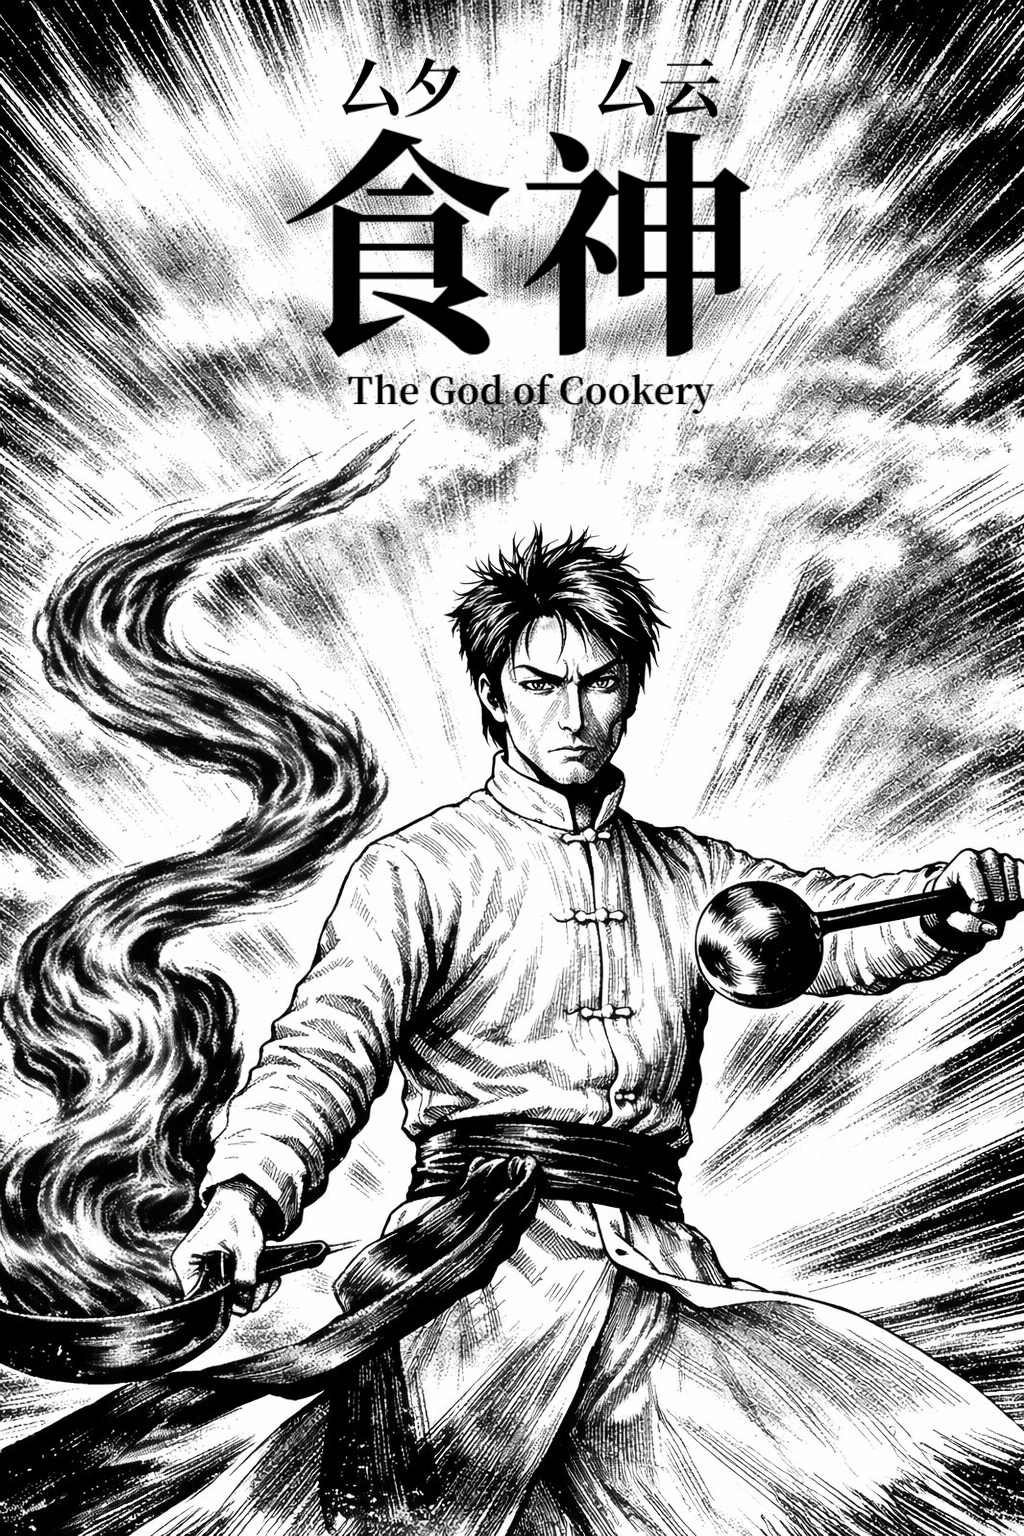
\includegraphics[width=4in]{../pics/god-of-cookery-final.png}};

  % Title line below image (front panel): 食神劇本全文 + Jyutcitzi + 註音
  \node[anchor=center, font=\Large\bfseries, black, align=center] at (9.373,1.5) {\jcz{}食神劇本全文註音};
  

  % 8) Bleed reminder
  % \node[anchor=south, font=\tiny\sffamily, gray] at (6.249,0.06) {Bleed 0.125'' | Trim 6''$\times$9'' | Spine 0.248'' (110 pp)};
\end{tikzpicture}

\end{document}
